%%%%% 数値例%%%%%%%%%%%%%%%%%%%%%%%%%

%\chapter{不良部品の検査,廃棄タイミング} \label{sec:chapter4}
%
%
%\chaptermark{不良部品の検査,廃棄タイミング}
%
%\section{不良部品の検査,廃棄タイミング\label{sec:rule}}
%検査,廃棄を行う目的は,システムの途中で不良部品の廃棄を行うことにより,各工程における不良部品のバッファの占有率を下げることである.
%よって,FFSの性能評価をするために,不良部品が発生する場合その検査及び廃棄をするタイミングが重要となる.
%本章では不良部品の検査・廃棄を行う工程数を一つから二つに増やしたとき,スループットの低下率が最も小さくなる工程の組み合わせについて考える.
%ここでは各工程における検査,廃棄のタイミングは次の工程のバッファに入る前,つまり各工程の処理直後に行うものとする.
%ただし,マッチング処理制約の影響がある第3工程では,一方のラインで不良部品が発生した場合でも第4工程のバッファに送り,第4工程でペアが揃ったとき,いずれかが不良部品であれば廃棄する.
%また,検査されることなく次の工程に送られた不良部品は次の工程において必ず不良部品となるものとした.
%各工程におけるバッファの大きさは,二つの別々のラインを持つ第1工程と第3工程は処理中の部品を含めずに1,二つの部品の組み合わせのある第2工程と第4工程における各部品のバッファをそれぞれ2とした.
%
%検査を行える位置は第1工程直後,第2工程直後,第3工程後,第4工程直後の四つである.
%検査を行う工程を選ぶ条件として,最終的なシステムからの離脱を考える第4工程の直後では必ず検査を行うものとする.
%まず,検査を行う工程の数を一つとしたとき,条件より考えられる検査工程のパターンは,第4工程で組み合わせた直後に検査を行うパターンのみである.
%次に,検査を行う工程の数を二つとしたとき,条件より考えられる検査工程のパターンとしては,”第1工程直後と第4工程直後”,”第2工程直後と第4工程直後”,”第3工程後と第4工程直後”の三つのパターンである.
%
%図 \ref{fig:ffs4}が第4工程の直後のみ検査を行う場合のGSPNである.
%次に図 \ref{fig:ffs14},\ref{fig:ffs24},\ref{fig:ffs34}は前節で述べた検査を行う工程数を二つとしたときの三つの待ち行列ネットワークに対応するGSPNである.
%いずれのGSPNも,各部品の処理の成否を記憶する必要があるため,第 \ref{sec:chapter3} 章で利用したGSPNより状態数が増えている.
%これらのGSPNを用いて,性能評価を行う.

\chapter{Inspection and removal timing of defective parts \label{sec:chapter4}}

\chaptermark{Inspection and removal timing of defective parts}

\section{Inspection and removal timing of defective parts \label{sec:rule}}
The purpose of inspection and removal is to reduce occupation ratio of buffers of defective parts in each process by discarding defective parts in the middle of the system.
Therefore, to evaluate the performance of FFS, the timing of inspection and removal when defective parts occurs is important.
We assume that inspection is done at not all the step but in specific step.
In this chapter, we consider the combination of steps that make the decrease rate of the throuput least when the number of inspection and removal of defective parts is increased from one to two.
The timing of inspection and removal in each step is performed before entering the buffer of the next step, that is, immediately after the processing of each step.
However, for the third step which is affected by the match processing constraint, if the defective parts occurs in one line, it is not immediately removed and sent to the buffer of the fourth step. When the pair is completed in the fourth step, if either of parts were defective one, remove.
Also, defective parts that were sent to the next step without being inspected will always make defective parts in the next step.
We set the size of buffer for first and third step, which has two separate line, to be 1 and second and fourth step, which has combination process, to be 2.

The place where the inspection can be performed are immediately after first, second, fourth step and after third step, which is before combination process at fourth step.
As a requirement for selecting the step to be inspected, the inspection has to be done immediately after fourth step where parts finally leave the system.
Therefore, if we set number of inspection to 1, the pattern of the inspection step considered from the requirement is only the one when inspection is done immediately after fourth step.
If we set the number of step to be inspected to 2, the pattern of the inspected step considered from the requirement is "immediately after the first and fourth step", "immediately after the second and fourth step", and "after the third steo and immediately after the fourth step."

Figure $\ref{fig:ffs4}$ shows the GSPN when inspection is done immediately after fourth step only.
Figure $\ref{fig:ffs14}$, $\ref{fig:ffs24}$, $\ref{fig:ffs34}$ shows the GSPN corresponding to the three queuing network of the three pattern we suggested above.
Since each GSPN needs to memorize the success or failure of the processing of each step, the number of states is increased more than the GSPN used in chapter $\ref{sec:chapter3}$.
We do performance evaluation using these GSPNs.


%\section{数値実験 \label{sec:compute2}}
%”第4工程直後”,”第1工程直後と第4工程直後”,”第2工程直後と第4工程直後”,”第3工程後と第4工程直後”の合計四つのパターンに対し性能指標としてスループットとブロッキング確率,及びスループットの低下率の計算をおこなう.
%%あやしい低下率の解説
%低下率は,不良率が$0\%$であるときを基準として,不良率を変化させたときのスループットの減少を示す値であり,以下の式によって求められる.
%\begin{eqnarray*}
%\mbox{decrease rate} = \frac{(\mbox{$\beta=0$のスループット})-(\mbox{$\beta$変化後のスループット})}{\mbox{$\beta=0$のスループット}} \times 100
%\end{eqnarray*}
%本研究では検査工程数の増加がスループットに与える影響を調べたい.
%そのため,予め単一の製品が正常に加工される確率(第4工程直後だけで不良部品を廃棄する場合のスループットの低下率と同じ)を計算し,その値を基準として検査工程数を増やしたとき,どの程度低下率が改善されるのかという評価を行う.
%基準となる低下率は以下の表 \ref{tb:base} のようになる.
%%低下率の解説終了
%スループットは単位時間あたりに第4工程で処理される部品数で定義する.
%ブロッキング確率は,定常状態において各工程のバッファに空きがない状態の確率を算出する.
%2種類の部品に対して同じ到着率,処理率を仮定しているため,第1及び第3工程の一方のラインだけに注目し,そのブロッキング確率を算出している.
%
%以上の条件の元で,各工程の処理率$\mu = 1.0$,部品の到着率$\lambda = 0.7$及び$\lambda = 0.3$のとき,不良率$\beta$を変動させ,各パターンにおけるスループットとブロッキング確率,低下率の三つの要素を計算した結果が表 \ref{tb:1} から表 \ref{tb:8}である.
%各工程におけるブロッキング確率をn-BP(n=1,2,3,4)と表している.

\section{Numerical experiment \label{sec:compute2}}
For performance measure, we calculate throughout, blocking probability, and decrease rate of throuput for four patterns of combination of steps to be inspected.
The four patterns are "immediately after fourth step.", "immediately after the first and fourth step", "immediately after the second and fourth step", and "after the third steo and immediately after the fourth step."
Decrease rate is a value indicating a decrease in throughput when the failure rate is changed with value when failure rate is $0\%$ as a standard and it is obtained by following formula.
\begin{eqnarray*}
\mbox{decrease rate} = \frac{(\mbox{throughput when $\beta=0$})-(\mbox{throughput after $\beta$ changed})}{\mbox{throughput when $\beta=0$}} \times 100
\end{eqnarray*}

In this paper, we want to investigate the influence of increase of number of step to be inspected on throughput.
Therefore, the probability of single product is processed normally (same as the decrease rate of throughput when removing defective parts immediately after fourth step) is calculated first, and using that probability as basis, when we increase the number of step to be inspected, we measure how decrease rate is improved.
The table $\ref{tb:base}$ shows the basis decrease rate.

The throughput is defined as the number of parts processed in the fourth steps per unit time.
Blocking probability calculates the probability of the buffer of each step to be full in steady state.
In this calculation of blocking probability, since the same arrival rate and processing rate are assumed for the two parts, attention is paid only to one line of the first and third step. 

We set processing rate of each process to $\mu=1.0$, arrival rate of parts to $\lambda =0.7$ and $\lambda = 0.3$.
Under the above conditions, we change failure rate $\beta$ and calculate throughput, blocking probability, and decrease rate for all four pattern.
The table $\ref{tb:1}$ to $\ref{tb:8}$ shows the result of experiment.
The blocking probability in each step is expressed as n-BP (n = 1, 2, 3, 4) and decrease rate is expressed as DR.

\begin{table}[ht]
	\centering
	\caption{Probability that parts leaving the system is defective}
	\scalebox{1.5}{
		\begin{tabular}{| l | l |} \hline
			$\beta$ & decrease rate($\%$) \\ \hline
			0 & 0	\\ \hline
			0.0001 & 0.060 \\ \hline
			0.01 & 5.85 \\ \hline
			0.02 & 11.4 \\ \hline
			0.03 & 16.7 \\ \hline
			0.04 & 21.7 \\ \hline
			0.05 & 26.5 \\ \hline
			0.1 & 46.9 \\ \hline
			0.5 & 98.4 \\ \hline
		\end{tabular}
	}
	\label{tb:base}
\end{table}





\begin{figure}[p]
\begin{center}
	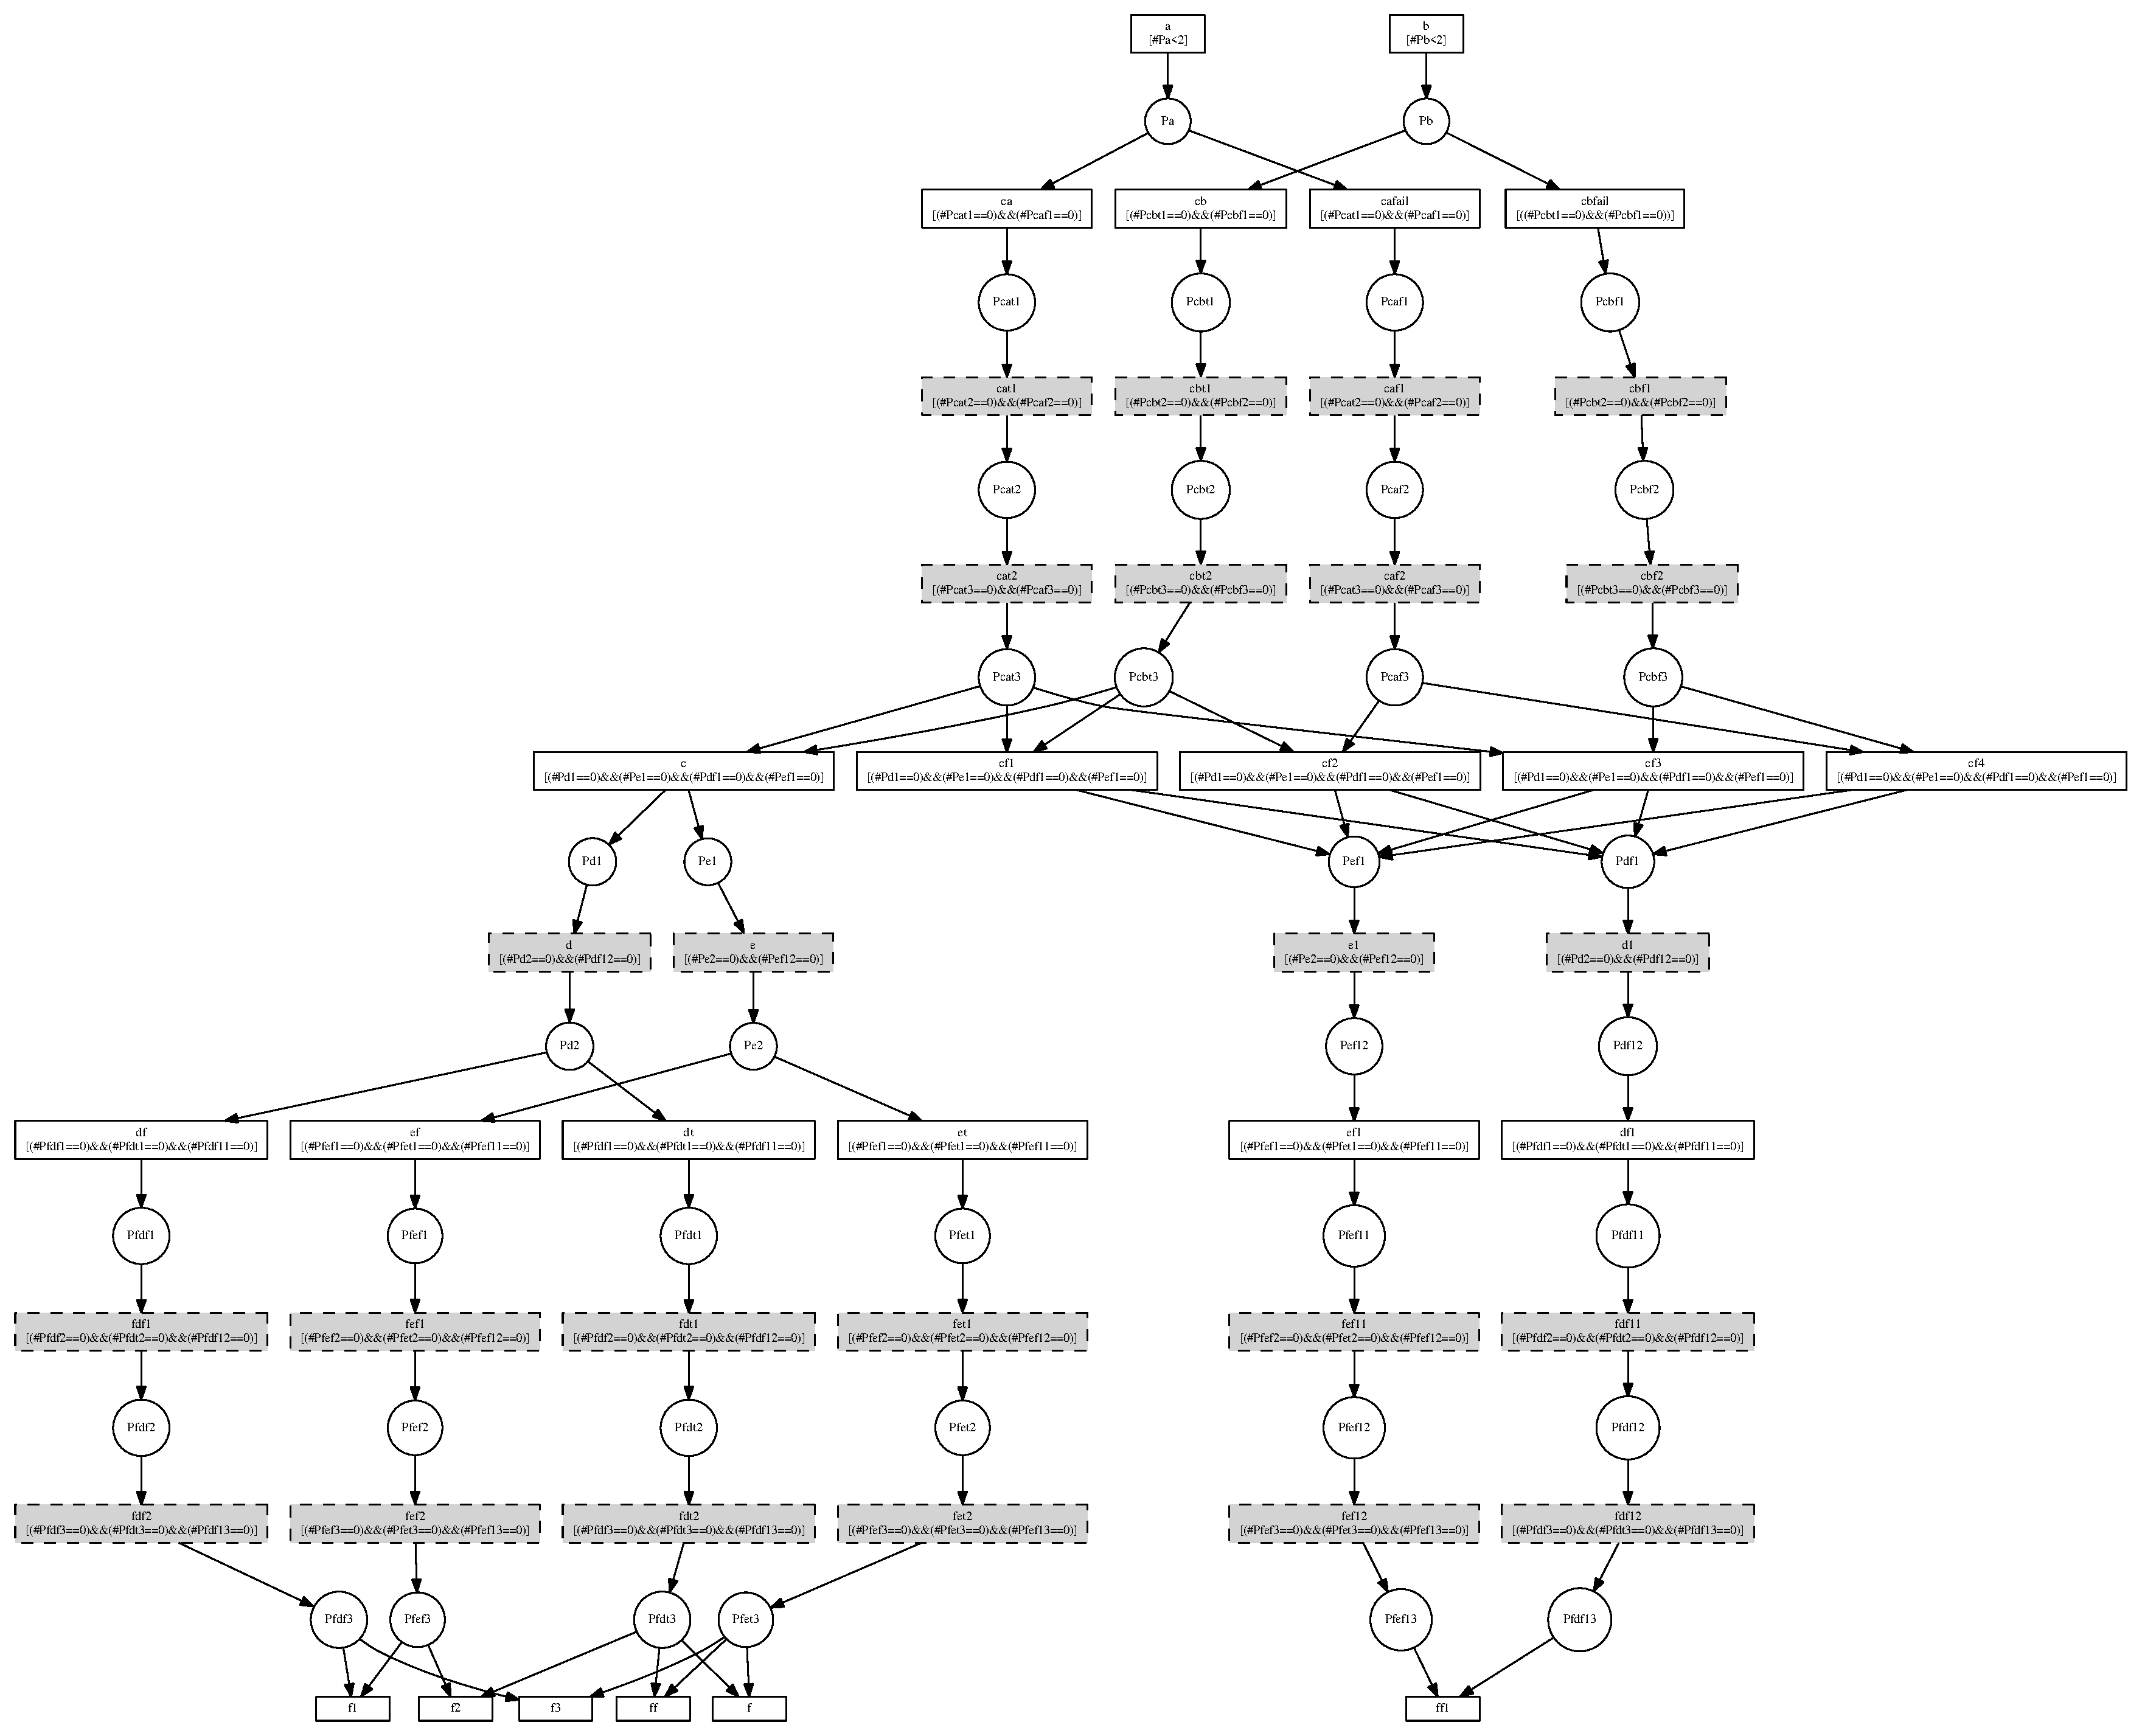
\includegraphics[width=\hsize]{fig/4a.eps}
\end{center}
\caption{GSPN for 4 step FFS with inspection done immediately after fourth step.}
\label{fig:ffs4}
\end{figure}

\begin{figure}[p]
\begin{center}
	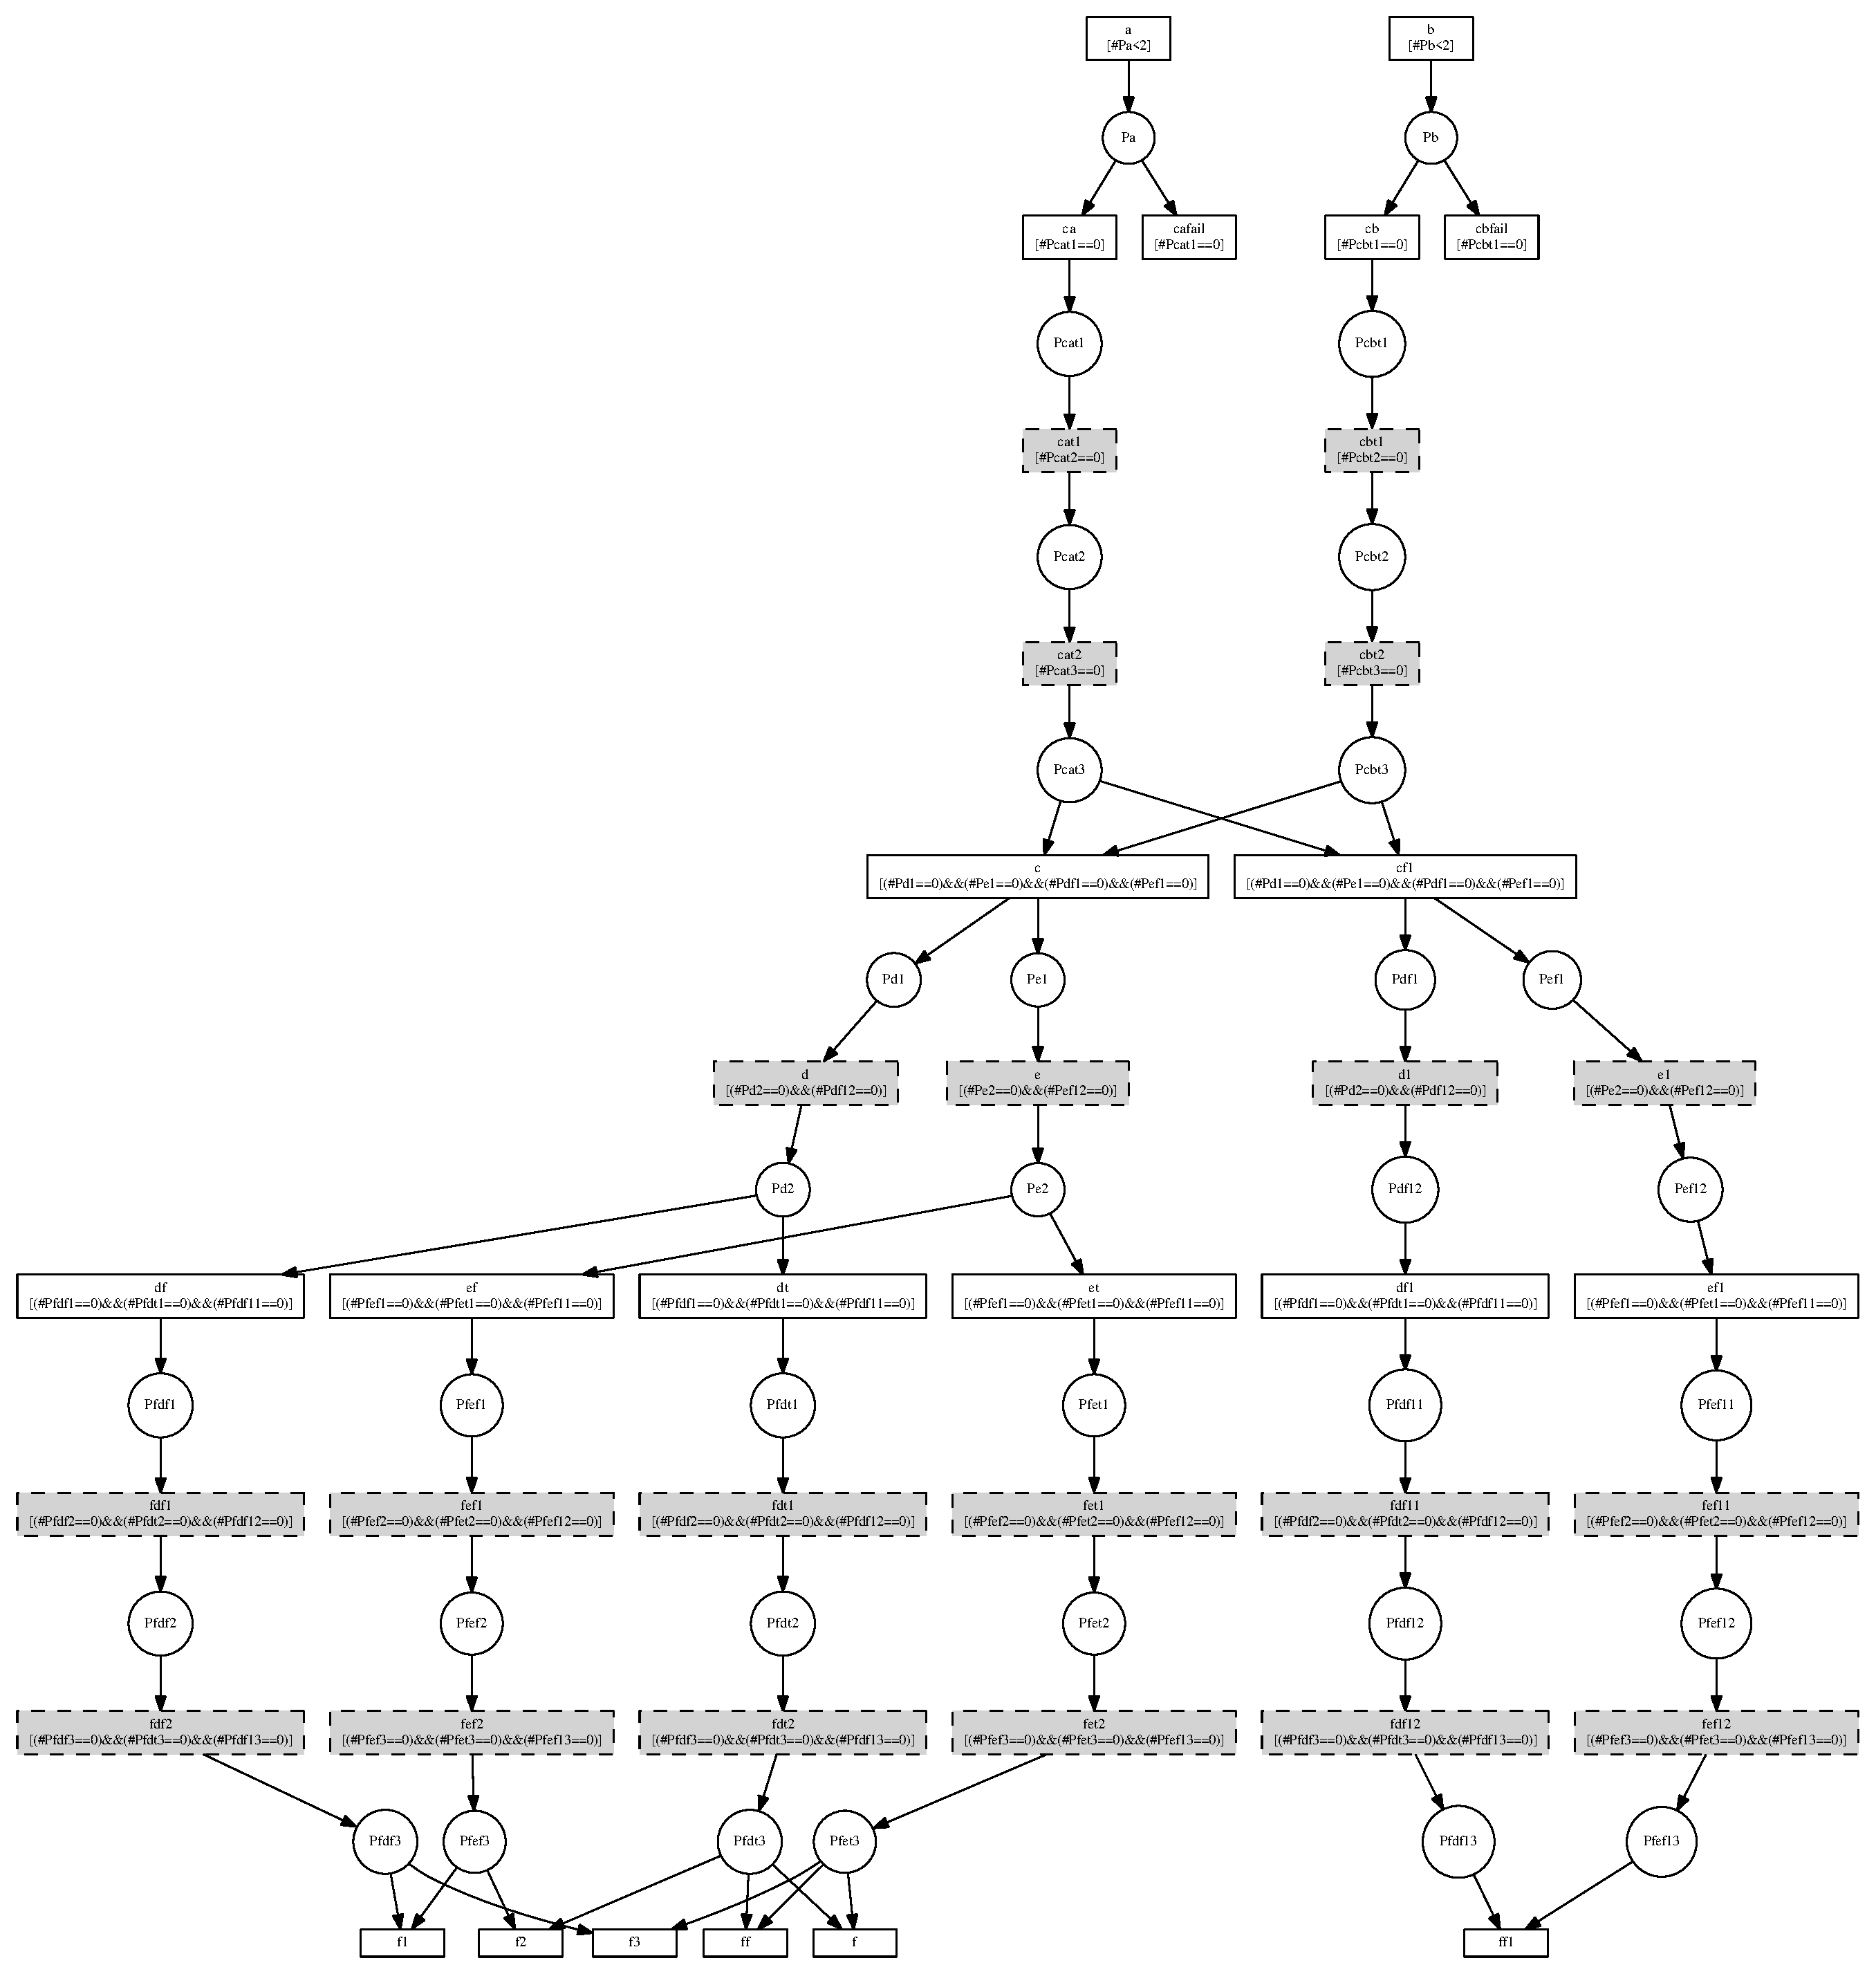
\includegraphics[width=\hsize]{fig/1a-4a.eps}
\end{center}
\caption{GSPN for 4 step FFS with inspection done immediately after first and fourth step.}
\label{fig:ffs14}
\end{figure}

\begin{figure}[p]
\begin{center}
	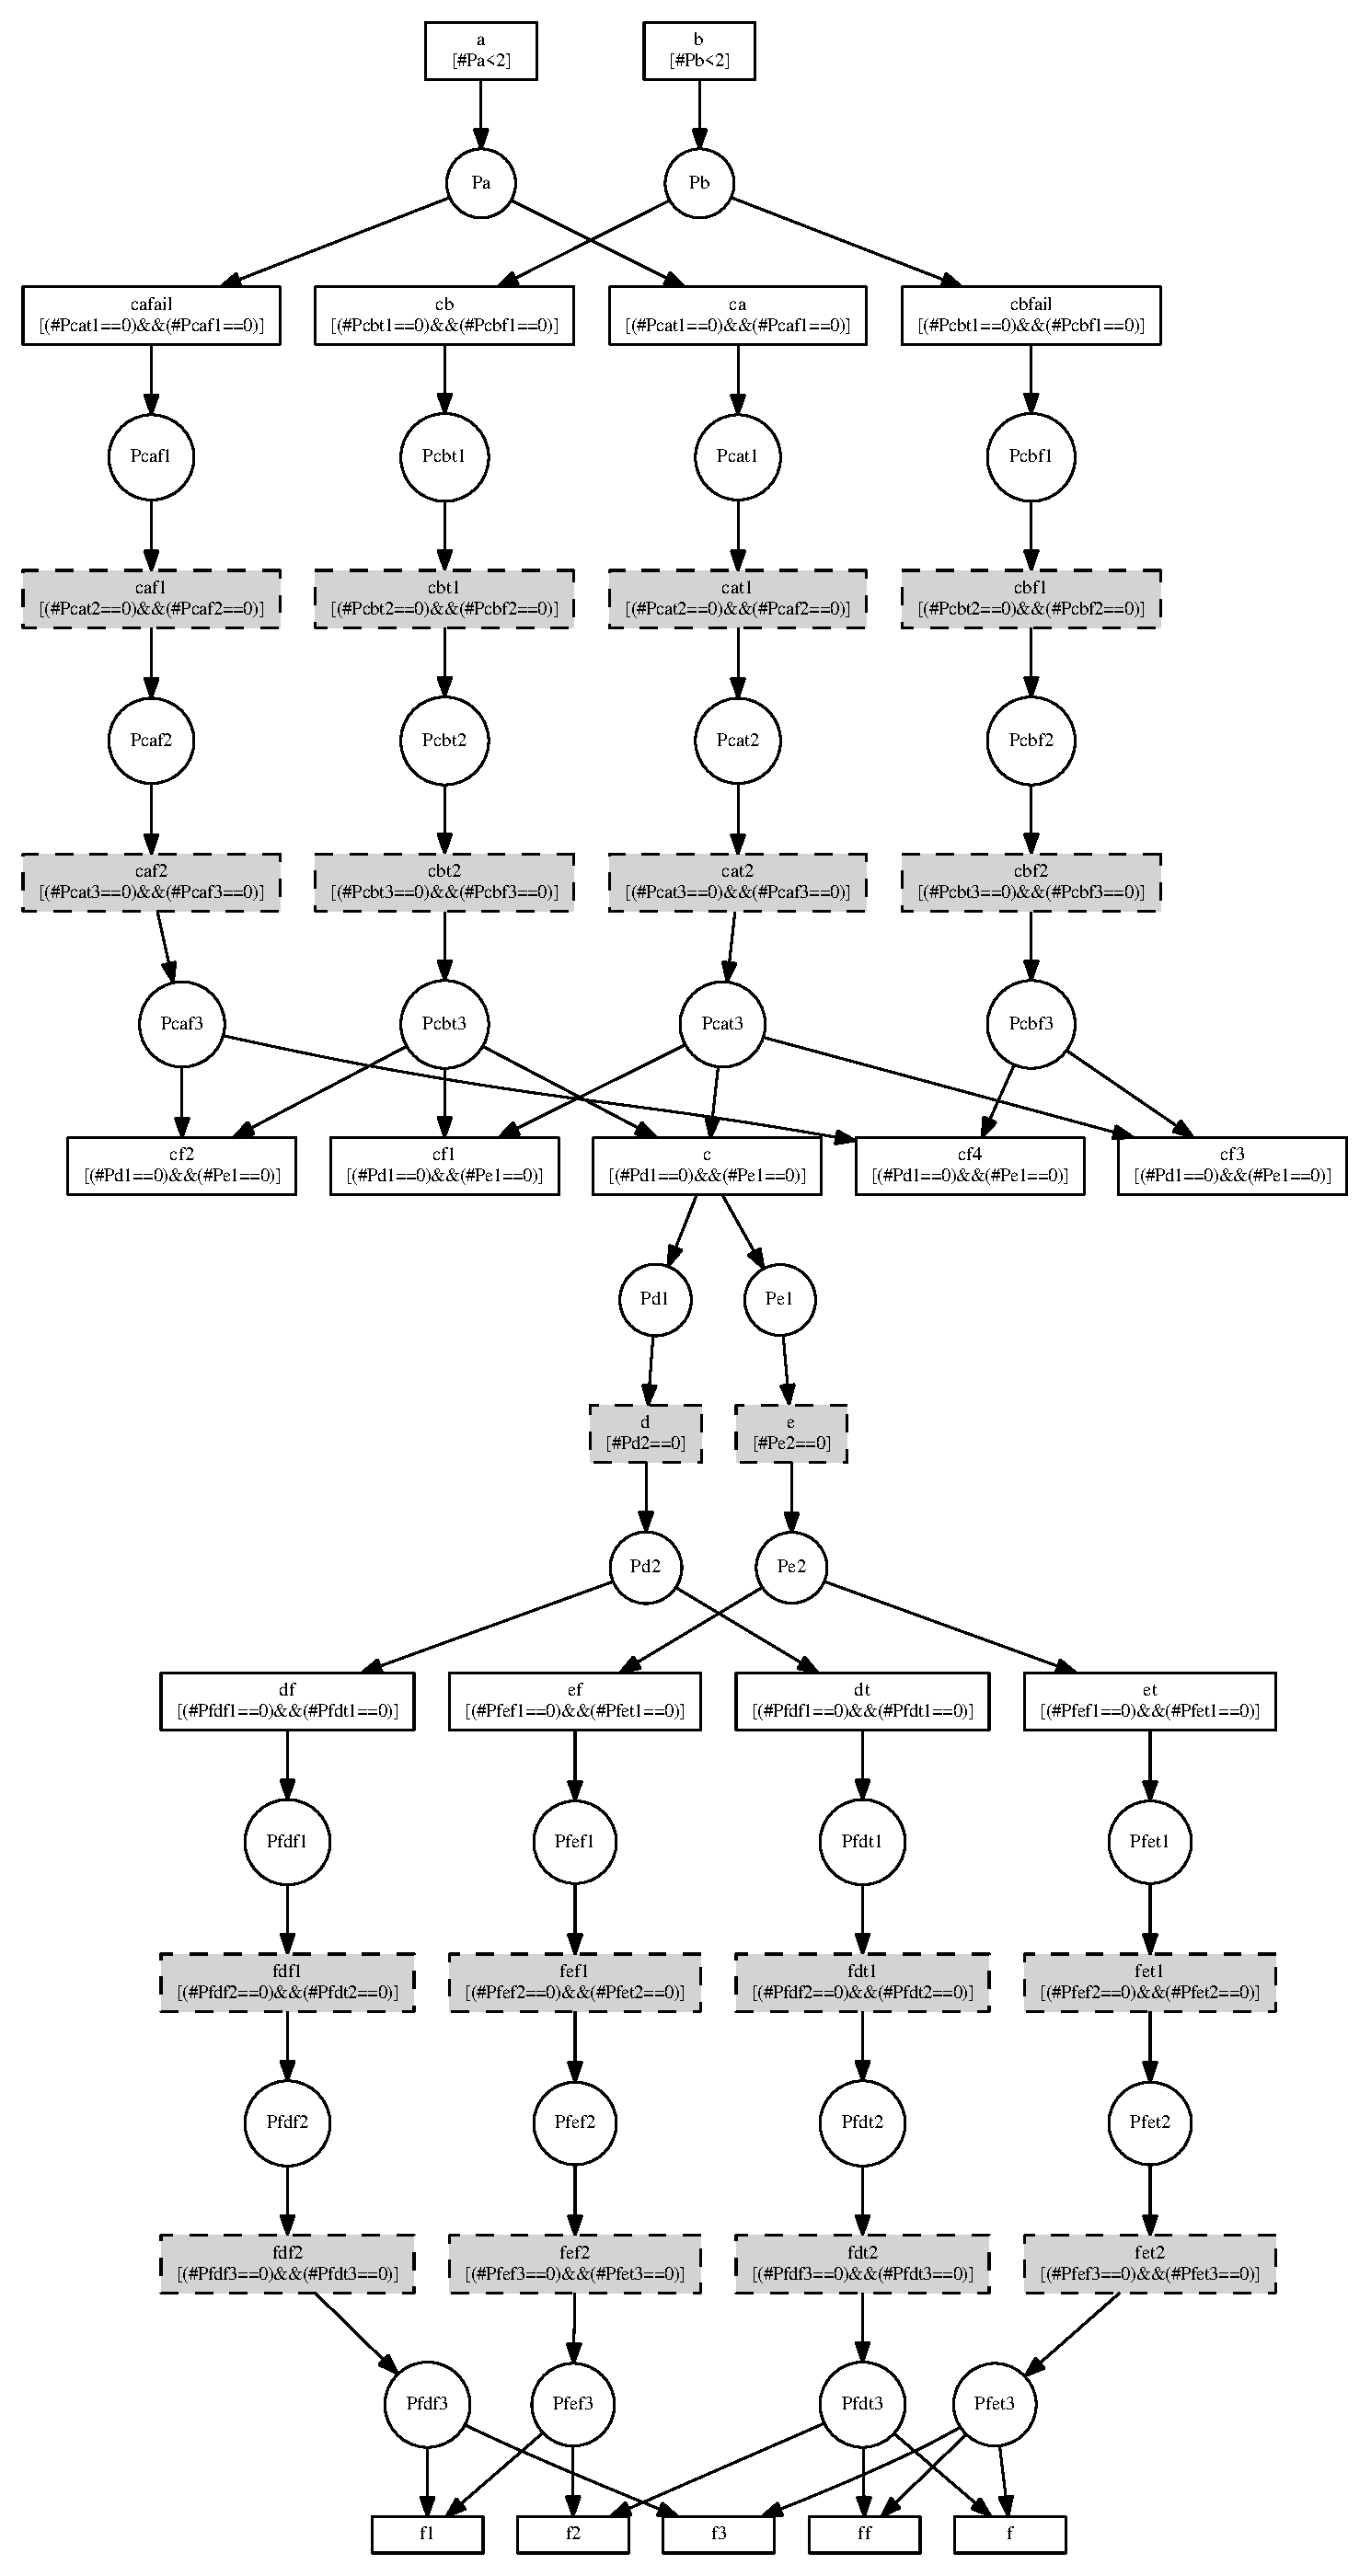
\includegraphics[height=\vsize]{fig/2a-4a.eps}
\end{center}
\caption{GSPN for 4 step FFS with inspection done immediately after second and fourth step.}
\label{fig:ffs24}
\end{figure}

\begin{figure}[p]
\begin{center}
	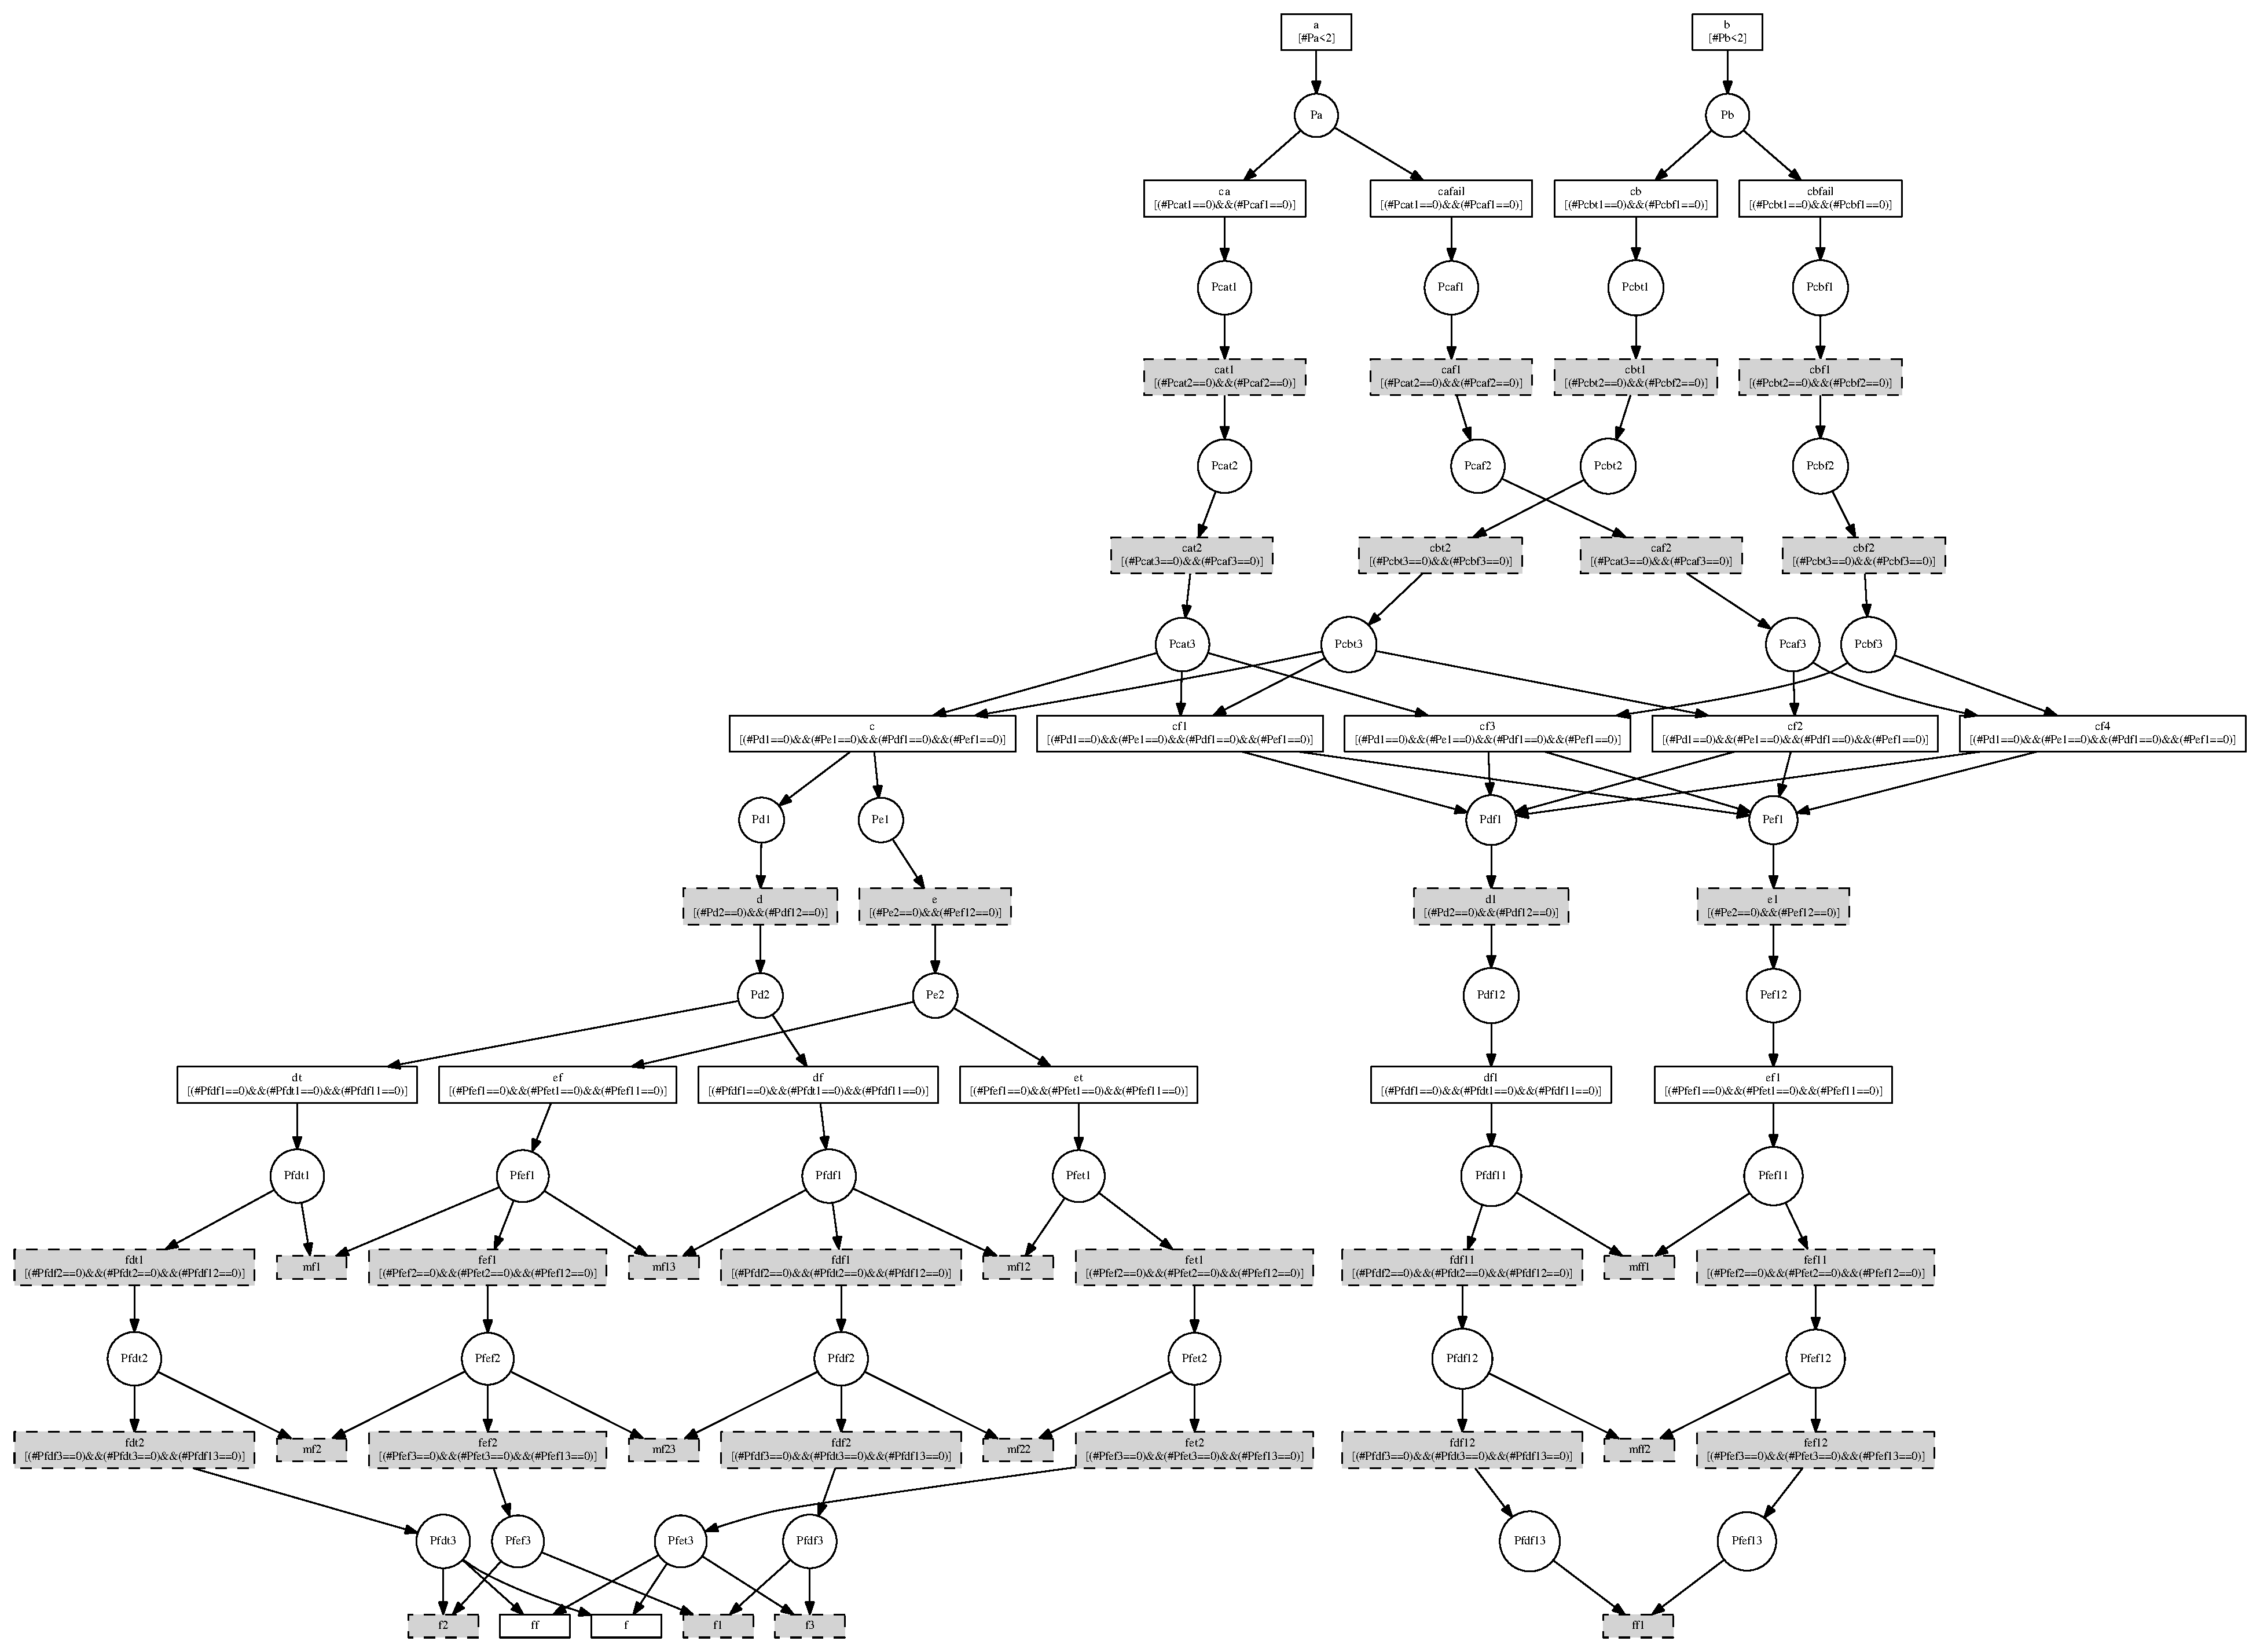
\includegraphics[width=\hsize]{fig/3a-4a.eps}
\end{center}
\caption{GSPN for 4 step FFS with inspection done after third step and immediately after fourth step.}
\label{fig:ffs34}
\end{figure}

\clearpage


%%%上から順に1,2,のときのスループットの値
\begin{table}[p]
	\centering
	\caption{Inspection done immediately after fourth step,$\lambda=0.7, \mu=1.0$}
	\scalebox{1.5}{
		\begin{tabular}{| l | l | l | l | l | l | l |} \hline
			$\beta$ & TP & 1-BP & 2-BP & 3-BP & 4-BP & DR($\%$) \\ \hline
			0.00 & 0.457 & 0.346 & 0.297 & 0.285 & 0.065 & 0 \\ \hline
			0.0001 & 0.456 & 0.346 & 0.297 & 0.285 & 0.065 & 0.060 \\ \hline
			0.01 & 0.430 & 0.346 & 0.297 & 0.285 & 0.065 & 5.85 \\ \hline
			0.02 & 0.404 & 0.346 & 0.297 & 0.285 & 0.065 & 11.4 \\ \hline
			0.03 & 0.381 & 0.346 & 0.297 & 0.285 & 0.065 & 16.7 \\ \hline
			0.04 & 0.357 & 0.346 & 0.297 & 0.285 & 0.065 & 21.7 \\ \hline
			0.05 & 0.336 & 0.346 & 0.297 & 0.285 & 0.065 & 26.5 \\ \hline
			0.1 & 0.243 & 0.346 & 0.297 & 0.285 & 0.065  & 46.9 \\ \hline
			0.5 & 0.007 & 0.346 & 0.297 & 0.285 & 0.065  & 98.4 \\ \hline
		\end{tabular}
	}
\label{tb:1}
\end{table}

\begin{table}[p]
	\centering
	\caption{Inspection done immediately after fourth step,$\lambda=0.3, \mu=1.0$}
	\scalebox{1.5}{
		\begin{tabular}{| l | l | l | l | l | l | l |} \hline
			$\beta$ & TP & 1-BP & 2-BP & 3-BP & 4-BP & DR($\%$) \\ \hline
			0.00 & 0.254 & 0.155 & 0.228 & 0.088 & 0.012 & 0 \\ \hline
			0.0001 & 0.253 & 0.155 & 0.228 & 0.088 & 0.01 & 0.060 \\ \hline
			0.01 & 0.239 & 0.155 & 0.228 & 0.088 & 0.012 & 5.85 \\ \hline
			0.02 & 0.225 & 0.155 & 0.228 & 0.088 & 0.012 & 11.4 \\ \hline
			0.03 & 0.211 & 0.155 & 0.228 & 0.088 & 0.012 & 16.7 \\ \hline
			0.04 & 0.198 & 0.155 & 0.228 & 0.088 & 0.012 & 21.7 \\ \hline
			0.05 & 0.186 & 0.155 & 0.228 & 0.088 & 0.012 & 26.5 \\ \hline
			0.1 & 0.135 & 0.155 & 0.228 & 0.088 & 0.012 & 46.9 \\ \hline
			0.5 & 0.003 & 0.155 & 0.228 & 0.088 & 0.012 & 98.4 \\ \hline
		\end{tabular}
	}
\label{tb:2}
\end{table}



\begin{table}[p]
	\centering
	\caption{Inspection done immediately after first and fourth step,$\lambda=0.7, \mu=1.0$}
	\scalebox{1.5}{
		\begin{tabular}{| l | l | l | l | l | l | l |} \hline
			$\beta$ & TP & 1-BP & 2-BP & 3-BP & 4-BP & DR($\%$) \\ \hline
			0.00 & 0.457 & 0.243 & 0.297 & 0.285 & 0.065 & 0 \\ \hline
			0.0001 & 0.457 & 0.243 & 0.297 & 0.285 & 0.065 & 0.048 \\ \hline
			0.01 & 0.435 & 0.242 & 0.292 & 0.280 & 0.064 & 4.67 \\ \hline
			0.02 & 0.415 & 0.241 & 0.288 & 0.276 & 0.063 & 9.17 \\ \hline
			0.03 & 0.395 & 0.240 & 0.293 & 0.271 & 0.061 & 13.5 \\ \hline
			0.04 & 0.376 & 0.239 & 0.279 & 0.266 & 0.060 & 17.7 \\ \hline
			0.05 & 0.358 & 0.238 & 0.275 & 0.261 & 0.058 & 21.7 \\ \hline
			0.1 & 0.276 & 0.233 & 0.256 & 0.237 & 0.051 & 39.7 \\ \hline
			0.5 & 0.015 & 0.223 & 0.176 & 0.073 & 0.009 & 96.7 \\ \hline
		\end{tabular}
	}
\label{tb:3}
\end{table}



\begin{table}[p]
	\centering
	\caption{Inspection done immediately after first and fourth step,$\lambda=0.3 \mu=1.0$}
	\scalebox{1.5}{
		\begin{tabular}{| l | l | l | l | l | l | l |} \hline
			$\beta$ & TP & 1-BP & 2-BP & 3-BP & 4-BP & DR($\%$) \\ \hline
			0.00 & 0.254 & 0.046 & 0.228 & 0.088 & 0.012 & 0  \\ \hline
			0.0001 & 0.253 & 0.046 & 0.228 & 0.088 & 0.012 & 0.050 \\ \hline
			0.01 & 0.241 & 0.047 & 0.227 & 0.086 & 0.012 & 4.93 \\ \hline
			0.02 & 0.229 & 0.047 & 0.226 & 0.084 & 0.012 & 9.66 \\ \hline
			0.03 & 0.218 & 0.047 & 0.225 & 0.072 & 0.011 & 14.2 \\ \hline
			0.04 & 0.206 & 0.047 & 0.225 & 0.080 & 0.011 & 18.6 \\ \hline
			0.05 & 0.196 & 0.047 & 0.224 & 0.079 & 0.010 & 22.7 \\ \hline
			0.1 & 0.149 & 0.047 & 0.219 & 0.070 & 0.008 & 41.1 \\ \hline
			0.5 & 0.008 & 0.051 & 0.192 & 0.020 & 0.001 & 96.9 \\ \hline
		\end{tabular}
	}
\label{tb:4}
\end{table}




\begin{table}[p]
	\centering
	\caption{Inspection done immediately after second and fourth step,$\lambda=0.7 \mu=1.0$}
	\scalebox{1.5}{
		\begin{tabular}{| l | l | l | l | l | l | l |} \hline
			$\beta$ & TP & 1-BP & 2-BP & 3-BP & 4-BP & DR($\%$) \\ \hline
			0.00 & 0.457 & 0.243 & 0.297 & 0.285 & 0.065 & 0 \\ \hline
			0.0001 & 0.456 & 0.243 & 0.296 & 0.285 & 0.065 & 0.056 \\ \hline
			0.01 & 0.432 & 0.241 & 0.291 & 0.269 & 0.060 & 5.48 \\ \hline
			0.02 & 0.408 & 0.239 & 0.285 & 0.254 & 0.056 & 10.7 \\ \hline
			0.03 & 0.385 & 0.238 & 0.280 & 0.239 & 0.052 & 15.8 \\ \hline
			0.04 & 0.363 & 0.236 & 0.276 & 0.225 & 0.047 & 20.6 \\ \hline
			0.05 & 0.342 & 0.235 & 0.272 & 0.212 & 0.044 & 25.3 \\ \hline
			0.1 & 0.250 & 0.230 & 0.255 & 0.155 & 0.028 & 45.4 \\ \hline
			0.5 & 0.007 & 0.221 & 0.221 & 0.005 & 1.62E-4 & 98.4 \\ \hline
		\end{tabular}
	}
\label{tb:5}
\end{table}


\begin{table}[p]
	\centering
	\caption{Inspection done immediately after second and fourth step,$\lambda=0.3 \mu=1.0$}
	\scalebox{1.5}{
		\begin{tabular}{| l | l | l | l | l | l | l |} \hline
			$\beta$ & TP & 1-BP & 2-BP & 3-BP & 4-BP & DR($\%$) \\ \hline
			0.00 & 0.254 & 0.047 & 0.228 & 0.088 & 0.012 & 0 \\ \hline
			0.0001 & 0.253 & 0.046 & 0.228 & 0.088 & 0.012 & 0.060 \\ \hline
			0.01 & 0.239 & 0.046 & 0.227 & 0.083 & 0.011 & 5.84 \\ \hline
			0.02 & 0.225 & 0.046 & 0.227 & 0.078 & 0.010 & 11.4 \\ \hline
			0.03 & 0.211 & 0.046 & 0.227 & 0.073 & 0.009 & 16.7 \\ \hline
			0.04 & 0.199 & 0.046 & 0.226 & 0.069 & 0.009 & 21.7 \\ \hline
			0.05 & 0.186 & 0.046 & 0.226 & 0.065 & 0.008 & 26.5 \\ \hline
			0.1 & 0.135 & 0.046 & 0.225 & 0.047 & 0.005 & 46.8 \\ \hline
			0.5 & 0.004 & 0.046 & 0.222 & 0.001 & 2.55E-5 & 98.4 \\ \hline
		\end{tabular}
	}
\label{tb:6}
\end{table}


\begin{table}[p]
	\centering
	\caption{Inspection done after third step and immediately after fourth step,$\lambda=0.7, \mu=1.0$}
	\scalebox{1.5}{
		\begin{tabular}{| l | l | l | l | l | l | l |} \hline
			$\beta$ & TP & 1-BP & 2-BP & 3-BP & 4-BP & DR($\%$) \\ \hline
			0.00 & 0.457 & 0.347 & 0.297 & 0.285 & 0.065 & 0 \\ \hline
			0.0001 & 0.457 & 0.347 & 0.297 & 0.285 & 0.0065 & 0.059 \\ \hline
			0.01 & 0.431 & 0.346 & 0.296 & 0.284 & 0.065 & 5.77 \\ \hline
			0.02 & 0.406 & 0.346 & 0.295 & 0.282 & 0.066 & 11.3 \\ \hline
			0.03 & 0.382 & 0.346 & 0.295 & 0.281 & 0.068 & 16.5 \\ \hline
			0.04 & 0.359 & 0.346 & 0.294 & 0.280 & 0.070 & 21.5 \\ \hline
			0.05 & 0.337 & 0.345 & 0.294 & 0.279 & 0.072 & 26.2 \\ \hline
			0.1 & 0.244 & 0.345 & 0.294 & 0.279 & 0.089 & 46.6 \\ \hline
			0.5 & 0.007 & 0.350 & 0.303 & 0.298 & 0.206 & 98.4  \\ \hline
		\end{tabular}
	}
\label{tb:7}
\end{table}


\begin{table}[p]
	\centering
	\caption{Inspection done after third step and immediately after fourth step,$\lambda=0.3 \mu=1.0$}
	\scalebox{1.5}{
		\begin{tabular}{| l | l | l | l | l | l | l |} \hline
			$\beta$ & TP & 1-BP & 2-BP & 3-BP & 4-BP & DR($\%$) \\ \hline
			0.00 & 0.254 & 0.155 & 0.228 & 0.088 & 0.012 & 0 \\ \hline
			0.0001 & 0.253 & 0.155 & 0.228 & 0.088 & 0.012 & 0.060 \\ \hline
			0.01 & 0.239 & 0.155 & 0.228 & 0.088 & 0.015 & 5.85 \\ \hline
			0.02 & 0.225 & 0.155 & 0.228 & 0.088 & 0.018 & 11.4 \\ \hline
			0.03 & 0.211 & 0.155 & 0.228 & 0.087 & 0.021 & 16.7 \\ \hline
			0.04 & 0.198 & 0.155 & 0.228 & 0.087 & 0.024 & 21.7 \\ \hline
			0.05 & 0.186 & 0.155 & 0.228 & 0.087 & 0.026 & 26.5 \\ \hline
			0.1 & 0.135 & 0.155 & 0.228 & 0.087 & 0.041 & 46.9 \\ \hline
			0.5 & 0.004 & 0.155 & 0.228 & 0.086 & 0.113 & 98.4 \\ \hline
		\end{tabular}
	}
\label{tb:8}
\end{table}

\clearpage

%\section{考察}
%表\ref{tb:3}から表\ref{tb:8}より,検査工程数を一つから二つに増やしたとき,基準となる表 \ref{tb:base}の低下率と比較して,全てのパターンにおいて低下率が低くなっていることが分かる.
%これは,システム途中で不良部品を廃棄することによりバッファに空きを作ることで,ブロッキングの発生確率が抑えられているためだと考えられる.
%また,検査工程数が二つの3パターンの中で,低下率が最も小さくなるのは第1工程直後と第4工程直後に検査工程を設定した場合であった.
%この理由としては,不良部品は次の工程に送られるとそれ以降の工程で不良部品を生むという条件が影響していると考えられる.
%第1工程直後と第4工程直後で検査をする場合,第1工程の一方のラインで不良部品が発生した場合,もう一方のラインに影響はなく,廃棄されるのは一つの不良部品である.
%それに対し,組み合わせやマッチング処理制約のある第2工程以降では,第1工程から送られた部品のうち片方の部品が正常な部品であっても,もう一方が不良部品であれば正常な部品も不良部品とともに廃棄されてしまう.
%このように正常な部品も廃棄されているケースが多いことから,その他の二つのパターンではスループットのが低下率に変化が少ないと考えられる.
%
%以上のことから,検査工程数を増やすとスループットの低下率が下がり,スループットが高くなるという結果が得られた.
%また,この4工程FFSにおいて検査工程数が2つであるとき,不良部品は第1工程直後と第4工程直後においてFFSから取り除くと,最もスループットが高くなるという結果も得ることができた.

\section{Lessons learned}
From table $\ref{tb:3}$ to $\ref{tb:8}$, we can see that when number of inspected step increased from one to two, decrease rate in all pattern is lower compared to the decrease rate of the basis table $\ref{tb:base}$.
Thisi is considered to be because the blocking probability is lowered by making vacancies in the buffer by removing defective parts in the middle of the system.
Also, among the three patterns of having two inspection step, the decrease rate is the smallest when the inspction was set immediately after first and fourth step.
We can consider the reason for this is because of the following assumption, defective parts sent to next step will make parts defective in later step.
When inspection is done immediately after first and fourth step, when a defective part occurs in one line of the first step, there is no influence on the other line, and only one defective part is removed.
In contrast, after second step where combination and match processing constraint affect, even if one of the part sent from first step is normal, if the other part of the pair is a defective part, a normal part is also removed together with defective part.
Since many normal parts are discarded in this way, it can be considered that the decrease rate of the throughput is small in the other two pattern.

For the lessons, we learned that increasing the number of inspection steps reduces the decrease rate in throuput and throughput will improve.
Moreover, when the number of inspection steps in this 4 step FFS was two, we can obtain that when defective parts are removed from the FFS immediately after first and fourth step, the throughput becomes the highest.








